\documentclass{article}

%% The amssymb package provides various useful mathematical symbols

\usepackage{amssymb}
\usepackage{microtype}
\usepackage{subfigure}
\usepackage{booktabs} % for professional tables
\usepackage{xr}
\usepackage{times}
\usepackage{float} % for figure placement
\usepackage{amsmath}
\usepackage{graphicx}
\usepackage{amsthm}
\usepackage{mathtools}


%%%%%%%%%%%%%%%%%%%%%%%%%%%%%%%%
% THEOREMS
%%%%%%%%%%%%%%%%%%%%%%%%%%%%%%%%
\theoremstyle{plain}
\newtheorem{theorem}{Theorem}[section]
\newtheorem{proposition}[theorem]{Proposition}
\newtheorem{lemma}[theorem]{Lemma}
\newtheorem{corollary}[theorem]{Corollary}
\theoremstyle{definition}
\newtheorem{definition}[theorem]{Definition}
\newtheorem{assumption}[theorem]{Assumption}
\theoremstyle{remark}
\newtheorem{remark}[theorem]{Remark}
 

% hyperref makes hyperlinks in the resulting PDF.

% If your build breaks (sometimes temporarily if a hyperlink spans a page)

% please comment out the following usepackage line and replace

% \usepackage{icml2021} with \usepackage[nohyperref]{icml2021} above.

\usepackage{hyperref}

% Attempt to make hyperref and algorithmic work together better:

\newcommand{\theHalgorithm}{\arabic{algorithm}}

% Use the following line for the initial blind version submitted for review:

\usepackage{icml2023}

 

\icmltitlerunning{On the Estimation of Gaussian Mixture Copula Models}

 

\begin{document}

\twocolumn[

\icmltitle{On the Estimation of Gaussian Mixture Copula Models}

 

\icmlsetsymbol{equal}{*}

 

\begin{icmlauthorlist}

\icmlauthor{Aeiau Zzzz}{equal,to}

\end{icmlauthorlist}

 

\icmlaffiliation{to}{Department of Computation, University of Torontoland, Torontoland, Canada}

\icmlcorrespondingauthor{Ashutosh Tewari}{ashutosh80@gmail.com}

 

% You may provide any keywords that you

% find helpful for describing your paper; these are used to populate

% the "keywords" metadata in the PDF but will not be shown in the document

\icmlkeywords{Copulas, Density estimation, Normalizing flows, Mixture models}

 

\vskip 0.3in

]

 

\DeclareRobustCommand{\nativellDenom}[1] {\prod\limits_{r=1}^{d}\psi_{r}\left(\Psi^{-1}_{r} \left( \bs{u}_r{#1} \right);\Theta^r \right) }

\DeclareRobustCommand{\llDenom}[1] {\prod\limits_{r=1}^{d}\psi_{r}\left(Z_{r{#1}};\Theta^r \right) }

\DeclareRobustCommand{\invCDF}[1]{ Z_{#1} }

\DeclareRobustCommand{\erf}{\textmd{erf}}

\DeclareRobustCommand{\AltllDenom}[1] {\log \left( \psi_{r}\left(\Psi^{-1}_{r} \left( \bs{u}_{r#1} \right);\Theta^r \right) \right) }

\DeclareRobustCommand{\zbar}[1] {\bar{Z}_{:{#1}}}

\DeclareRobustCommand{\ma_zbar}[2] {\bar{\textbf{z}}_{#1}(#2)}

\DeclareRobustCommand{\der}[2] {\frac{\partial \left({#2}\right)}{\partial {#1}}}

\newcommand{\bs}[1]{\boldsymbol{#1}}

\DeclareRobustCommand{\bf}[1]{\textbf{#1}}

\newcommand{\argmaxI}{\mathop{\mathrm{argmax}}\nolimits} % ASdeL

\printAffiliationsAndNotice{}  % leave blank if no need to mention equal contribution
%\printAffiliationsAndNotice{\icmlEqualContribution} % otherwise use the standard text.
\begin{abstract}

This paper revisits Gaussian Mixture Copula Model (GMCM), a more expressive alternative to the widely used Gaussian Mixture Model (GMM), to make its parameter estimation tractable. Both the Expectation Maximization and the direct Likelihood Maximization frameworks for GMCM have to grapple with a likelihood function that lacks a closed-form. This has led to a few approximation schemes that alleviate the problem, nonetheless leaving the issue still unresolved.  Additionally, past works have alluded to an additional challenge of parameter unidentifiability, but none has offered a rigorous treatment and a commensurate solution framework to overcome the same. This work offers solutions to each of these issues in an attempt to help GMCM realize its full potential. The source of unidentifiability is not only proven but also suitable priors are proposed that eliminate the problem. Additionally, an efficient numerical framework is proposed to evaluate the intractable likelihood function, while also providing its analytical derivatives. Finally, a view of GMCM as a series of bijective mappings from a base distribution is presented, which paves the way to synthesize GMCM using modern, probabilistic programming languages (PPLs). The main claims of this work are supported by empirical evidence gathered on synthetic and real-world data sets.

 

% a likelihood function that lacks a closed-form representation, and the reliance on numerical gradients (of likelihood function) make the parameter estimation cost prohibitive and impractical for high-dimensional, high-volume data-sets.

 

 

% for modeling continuous, multivariate data-sets, exhibiting multimodal distribution. GMCM combines the complex dependencies  endowed to Like other copula-based models, the strength of GMCMs comes from the ability to separate the learning of marginal models of the random variables from that of the dependence between them. Despite this flexibility and its potential impact on modeling real-world data, the learning of GMCM parameters is hard. The issue of non-identifiability, an intractable likelihood function that lacks a closed-form representation, and the reliance of maximum-likelihood methods on numerical gradients make the parameter estimation cost prohibitive and impractical for high-dimensional problems. This work offers solutions to each of these issues in an attempt to help GMCM realize its full potential. The main claims of this work are supported with empirical evidences shown on simulated and real-world data-sets.

\end{abstract}

 

%% \linenumbers

 

%% main text

\section{Introduction}\label{sec:Intro}

Modeling multivariate data is of fundamental interest, in several domains, to solve myriad of practical problems. From a probabilistic viewpoint, it amounts to defining a generative process that best explains the observed data when seen as random variables. Copulas provide a unique framework to model multivariate data that allows for complete control on the marginal behaviors of the random variables while being able to separately capture the dependencies between them. See \citep{Durante2010CopulaIntro} and references therein for a survey on this subject.  The decoupling $-$of marginal and joint behavior$-$ induced by a copula can be especially significant when the true data-generating process imposes strict constraints over the marginal distributions of some or all random variables. Ideally, any effort to model such data should adhere to these constraints. However, in the pursuit of finding a joint model of the random variables, one typically ends up with inconsistent marginal models.  Given the ability of copulas to overcome such inconsistencies, they have been applied in many scientific fields though particularly in finance \citep{Genest2009CopulaInFinance,Cherubini2004copula}, reliability analysis \citep{Rychlik2010Reliability} and molecular biology \citep{Bilgrau2012quantification,Li2011,Kim2008,Ma2012Gini}.  There have also been  attempts to find synergies between copula theory and machine learning to build high-fidelity data-driven models \citep[see][for a survey on the applications of copulas in machine learning approaches]{Elidan2013}.

The focus of this paper is on the multivariate modeling of continuous random variables, exhibiting multimodal behavior in their  joint (and/or marginal) distribution. Gaussian Mixture Models (GMMs) \citep{Bilmes98agentle} have been prolifically used to model such data sets, thanks to their simplicity and an efficient Expectation-Maximization (EM) algorithm for parameter estimation. However, the assumption of jointly normally distributed components is frequently violated in real-world applications, with unintended practical ramifications. The Gaussian mixture copula model (GMCM) \citep{Tewari2011,Bilgrau2016,Bhattacharya2014, kasa2018} offers a more expressive alternative to GMM while keeping the same parameterization to capture multimodal dependence structure. Figure \ref{fig:motivating_example_gmcm} illustrates the expressivity endowed by the GMCM via a synthetic two-dimensional data set with 100 samples (Figure \ref{fig:motivating_example_gmcm}a) that appears to have a bimodal distribution with non-Gaussian modes. The best-fit GMCM and a GMM are obtained on this data set, wherein the optimal number of components is determined via the widely used Bayesian Information Criterion (BIC). A quick look at the density contours (Figure \ref{fig:motivating_example_gmcm}b-\ref{fig:motivating_example_gmcm}c) and the generated random samples (Figure \ref{fig:motivating_example_gmcm}d-\ref{fig:motivating_example_gmcm}e), suggests that the GMCM is a more faithful model of the underlying data, with a noticeable tighter fit. The GMM, on the other hand, can be seen to diffuse into regions with no data support, even with an extra mixing component.

\begin{figure}[ht]
\centering
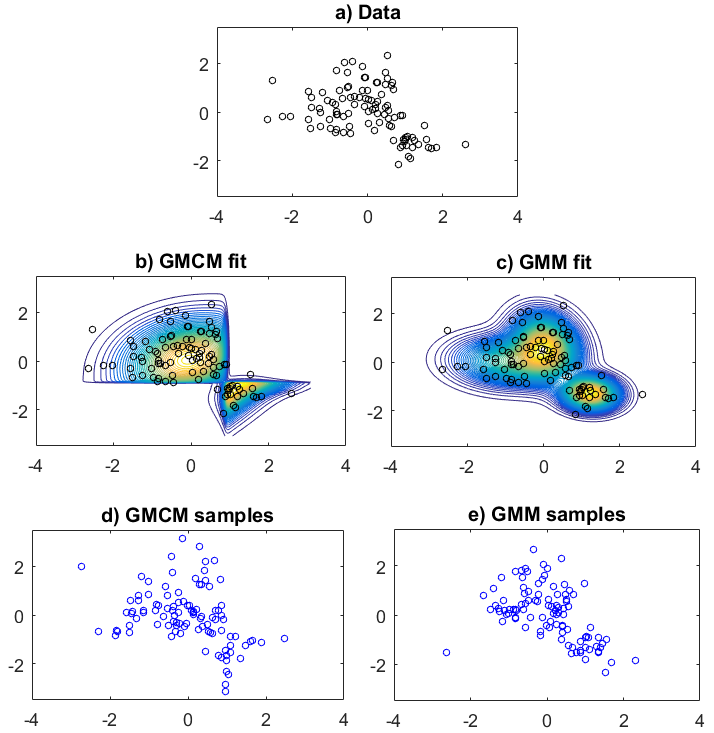
\includegraphics[width= 240pt,height=275pt]{figures/figure_for_motivating_gmcm}
\caption{(a) A 2-dimensional data set with 100 samples, (b-c) contours of best-fit GMCM (with 2 components) and GMM (with 3 components), (d-e) 100 random samples generated from the two fitted distributions. A tighter fit and a closer resemblance of the random samples to the training data set suggest the GMCM to be a superior generative model of the data than the GMM.}
\label{fig:motivating_example_gmcm}
\end{figure}

Despite its superior expressivity, the estimation of GMCM parameters remains a challenge primarily due to three reasons that we briefly mention here and later explain. First, GMCMs suffer from an inherent issue of \emph{parameter unidentifiability}. Second, its likelihood function does not admit a closed analytical form, and thus not amenable to the EM framework for parameter estimation. Third, concomitant to the second reason, even direct likelihood maximization (via gradient-based methods) becomes hard due to the lack of analytical gradients (numerical gradients are computationally expensive). The main contributions of this paper address each of these issues (not in the same order) i.e. 1) additional conditions are specified that provably mitigate the unidentifiability of GMCM, 2) a correct formulation of EM algorithm for GMCM is presented, 3) a numerical scheme is proposed to approximate GMCM's likelihood function while providing analytical gradient for the same, and 4) a view of GMCM as a series of bijective mappings is presented that makes it amenable to modern probabilistic programming frameworks and leverage their built-in automatic differentiation capabilities.

The plan of this paper is as follows. Sections \ref{subsec:LitReview} presents a short literature review on multivariate copula construction. Section \ref{sec:GMC_description} describes the GMCM framework and highlights the challenges with the estimation of its parameters (Section \ref{subsec:MLE_GMCM}). A view of GMCM as a series of bijective mappings is presented in Section \ref{sec:GMCM_bijective}, wherein a numerical scheme is also proposed to obtain an intractable mapping (Section \ref{subsec:gmm_quantile}). The source of unidentifiability of GMCM is discussed in section \ref{sec:identifiability_GMCM} and a solution is proposed. A correct derivation of EM algorithm for GMCM is presented in Section \ref{sec:EM}. Results on synthetic data sets are included in section \ref{sec:Experimental} to corroborate the claims, before concluding in section \ref{sec:Discussion} with remarks on a few future research directions.

\subsection{Multivariate Copula Construction}\label{subsec:LitReview}
The literature on copulas has been dominated by bivariate copula models with a rich set of parametric families to choose from \citep{Nelsen1999introduction}. Although the idea of higher dimensional copula construction is not new \citep[see][]{Genest1995Multivariate, Joe1993Multivariate,Kojadinovic2010RpackageMVcopula}, the literature on it is relatively recent. For instance, \citet{Bedford2002,Kurowicka2009Book,Czado2010PairCopula} proposed  synthesis of multivariate copula from bivariate copulas by assuming a tree-structured dependency between the random variables. This idea was extended to directed acyclic graphs \citep[see][]{Elidan2010,Hanea2006CBN},  giving rise to \emph{Copula Bayesian Networks}. In high-dimensional settings, the recovery of a sparse inverse covariance structure of a Gaussian copula was studied by \citet{Liu2009} yielding  \emph{non-paranormal} models.

Copula-based construction to address multi-modality \textemdash \ a frequently observed trait in real-world data\textemdash was first addressed by \citet{Tewari2011} with the proposal of GMCM. \citet{Bilgrau2016} furthered this work by noting certain challenges with the parameter estimation of GMCM and proposed practical solutions for the same. This was coupled with an improved implementation of the model as an open-source package \citep{Bilgrau_Rpackage} in R. \citet{Rajan2016_GMCM_mixed_data} extended GMCM to construct flexible generative models for mixed (continuous and discrete) data-types. The role of automatic differentiation, to obtain gradients of GMCM's intractable likelihood function, was explored by \citet{Kasa2022}. Nevertheless, these works only partly addressed the fundamental issues of GMCM pertaining to parameter unidentifiability and the intractability of its likelihood function (and its gradient), thereby motivating this work.

Recently, there have been some interesting developments in the area of \emph{model-based clustering} using copulas \citep{Kosmidis2016,Mazo2017,Marbac2017,Rey2012_CopulaMixture}. The motivation there is to overcome the restrictive normality assumption by cleverly using copulas, from \emph{known} parametric families, to capture the dependence in each mixing component; for instance, the \emph{Gaussian Copula Mixture Model} (GCMM) \citep{Marbac2017} employs a Gaussian copula for the same. Although with very similar motivations (and names), the two lines of work (GMCM and GCMM) are fundamentally different, as the goal in GMCM is to seek a \emph{single} copula distribution to capture the entire multimodal dependence structure. 

Another related (albeit rather remotely) line of work pertains to deep generative models a.k.a \emph{normalizing flows} (NFs), which has garnered significant attention in the Machine Learning community \citep[see][for a comprehensive review on NFs]{Kobyzev2021}. The core idea behind NFs is to transform a simple base distribution, such as an isotropic Gaussian, via bijective mappings that are carefully crafted using deep neural networks. Endowed with such mappings, one can compose highly expressive generative models for continuous data, resulting in best-in-class performances for the task of multivariate density estimation. The similarities and dissimilarities are drawn between GMCM and the NF-based models.   

\subsection{Notation}\label{subsec:Notation}
Lowercase letters are used for scalars, lowercase boldface letters for vectors, uppercase letters for matrices, and Greek letters for model parameters or functions. Unless otherwise stated, vectors are column vectors. Subscripts are used to denote an element of a vector or a matrix. For example, $\bs{x}_i$ and $X_{ij}$ denote the $i^{th}$ and the $(i,j)^{th}$ elements of a vector $\bs{x}$ and a matrix $X$, respectively. Likewise, $X_{i:}$ (or $X_{:i}$) represents the $i^{th}$ row (or column) of a matrix $X$. Subscripts are also used to indicate dimension-specific functions. For instance, the marginal distribution, induced by a joint distribution $\Psi$, along the $j^{th}$ dimension is denoted as $\Psi_j$.  Superscripts are reserved to indicate parameter association. For example, $\Theta^i$ denotes parameters associated with some entity $i$. Table \ref{tab:symbol_glossary} in appendix \ref{apd:symbol_glossary} lists frequently appearing symbols in the paper for quick reference.

\section{Gaussian Mixture Copula Model}\label{sec:GMC_description}
\begin{definition} \label{def:GMC}
 A \emph{m}-component \emph{Gaussian Mixture Copula} (GMC) distribution, parameterized by $\Theta = \{\bs{\mu}^l, \Sigma^l, \alpha^l\}_{l=1}^m$, defines a joint distribution of a vector $\bs{u}$, whose constituent elements are uniformly distributed, i.e. $ \bs{u}_j \sim \text{Uniform(0,1)}, \  j\in \{1,2,\cdots d\}$. The GMC density function is given by Equation \eqref{eq:GMC_density}.
\end{definition}

\begin{align}\label{eq:GMC_density}
\zeta(\bs{u};\Theta) & = \left( \frac{\psi\left(\Psi^{-1}(\bs{u});\Theta\right)}{\nativellDenom{}} \right)
\end{align}

The symbol $\psi(\cdot;\Theta)$ denotes the joint density function of a GMM parameterized with $\Theta = \{\bs{\mu}^l, \Sigma^l, \alpha^l\}_{l=1}^m$, where $\bs{\mu}^l \in \mathbb{R}^d$, $\Sigma^l \in \mathbb{S}_+^d$ and $\alpha^l \in \mathbb{R}_+ \text{s.t.} \sum \alpha^l=1$ denote the mean vector, the covariance matrix and the mixing proportion of the $l^{th}$ component, respectively. The marginal densities induced by the GMM are denoted by $\psi_r(\cdot;\Theta^r)$, with $\Theta^r\subset \Theta$ being the subset of parameters corresponding to the $r^{th}$ dimension. Also, $\Psi_r(\cdot)$ $\left(\text{and} \ \Psi^{-1}_r(\cdot) \right)$ is the cumulative distribution function (and its inverse) of the GMM along the $r^{th}$ margin, and $\Psi^{-1}(\bs{u})=[\Psi^{-1}_1(\bs{u}_1), \cdots, \Psi^{-1}_d(\bs{u}_d)]$. This definition directly follows from the \emph{inversion method} of constructing copulas from any multivariate distribution (in this case, a Gaussian Mixture distribution) with continuous margins ~\citep[see][chapter 3]{Nelsen1999Chapter3}. Since all the elements of a sample $\bs{u}\in [0,1]^d$ from GMC distribution are uniformly distributed, one can transform those via arbitrary univariate quantile functions $F_j^{-1}(u_j;\lambda_j) \ (j\in \{1,2,\cdots d\} )$, with their respective dimension specific parameters $\lambda_j$s. This feature allows one to model the marginal and the joint behavior of a multivariate data set independently (a hallmark of any copula-based model construction).

\subsection{MLE challenges in GMCM}\label{subsec:MLE_GMCM}
Maximum Likelihood Estimation (MLE) in GMCM amounts to estimating both the copula parameters ($\Theta$ in Definition \ref{def:GMC}) and the marginal parameters  ($\lambda_js$) in conjunction. Nevertheless, a computationally efficient and consistent estimator proposed by \citet{Joe1996}, where the marginal distributions are learned first followed by the estimation of copula parameters, is quite pervasive in practice. Along the same lines, this paper also assumes the marginal distributions to be arbitrary but known and tackles the much harder problem of estimating the GMC parameters by maximizing the log-likelihood function $\ell_{\zeta}(\Theta|U)$ given by Equation \eqref{eq:gmcm_logL},
\begin{align} \label{eq:gmcm_logL}
\ell_\zeta(\Theta |U) &= \sum\limits_{i=1}^{n} \log \left[\zeta(U_{:i};\Theta)\right],
\end{align}
where the function $\zeta(\cdot)$ is the GMC density function given by Equation \eqref{eq:GMC_density}. Assuming that from a training dataset $X \in \mathbb{R}^{d \times n}$ the marginal distributions have been learned, the matrix $U \in [0 , 1]^{d\times n}$ can then formed after transforming the dataset $X$ via the learned marginal distribution functions i.e., $U_{j:}=F_j(X_{j:};\lambda_j), j\in\{1,2,\cdots,d\}$. Being a continuous and smooth function, $\ell_\zeta(\Theta |U)$ can be maximized using any gradient-based algorithm, however, the task is computationally expensive. The primary culprit is the inverse function $\Psi^{-1}$ appearing in the expression of $\zeta(\bs{u};\Theta)$, which doesn't admit a closed analytical form. To further elaborate, let's look at the cumulative distribution function (Equation \ref{eq:invCDF_GMM}) of a univariate  $m$-component Gaussian mixture, along the $r^{th}$ dimension (note that $\Theta^r=\{\alpha^l,\bs{\mu}_r^l, \Sigma_{rr}^l \}_{l=1}^m$).  It is easy to verify that the corresponding inverse, $\bs{z}_r=\Psi_r^{-1}(\bs{u}_r)$, cannot be written explicitly, thus necessitating a numerical solution for the same.
\begin{equation} \label{eq:invCDF_GMM}
\bs{u}_r=\Psi_r(\bs{z}_r;\Theta^r)= \frac{1}{2}\sum\limits_{l=1}^{m} \alpha^l \left[1 + \erf\left( \frac{\bs{z}_r-\bs{\mu}^l_r}{\sqrt{2\Sigma_{rr}^l}}\right) \right]
\end{equation} 
\citet{Bilgrau2016} proposed an efficient inversion scheme based on linear interpolation on a sufficiently sized grid and exploiting the fact that $\Psi_r(\bs{z}_r)$ is monotonic. Furthermore, they used an empirical approximation of the \emph{error function}, $\erf(\cdot)$, in Equation \ref{eq:invCDF_GMM}. Although, these measures alleviate some issues, obtaining $\Psi_r^{-1}(\bs{u}_r)$ remains the bottleneck in the evaluation of the likelihood function in Equation \eqref{eq:gmcm_logL}. The overall cost to evaluate this function for $n,d \gg m$ turns out to be $O(mdg + nd\log{g})$, where $g$ is the grid size used for interpolation. The first term is due to the cost involved in evaluating \eqref{eq:invCDF_GMM} on $g$ grid-points for $d$ dimensions. The second term is the cost of linear interpolation of $d$, $n$-dimensional vectors.  

Obtaining the partial derivatives of \eqref{eq:gmcm_logL}, for gradient-based MLE, w.r.t $\Theta^r$ is even more challenging. In addition to the fact that the likelihood function lacks a closed form, it comprises logarithms of summands with exponential terms in both numerator and denominator, thus, making the derivation of analytical derivatives nontrivial. As a result, prior works \citep{Tewari2011, Bilgrau2016} relied on finite difference (FD) approximation of the gradient of the GMCM log-likelihood function. Although effective for small problems, this scheme scales poorly with problem dimensions. To make this point clear, let us first understand the computational complexity of FD gradient approximation. Since the GMC distribution has $O(md+md^2)$ parameters, the complexity of FD approximation becomes $O(md^2C_{\ell(\Theta|U)})$ (for $d\gg m$), with $C_{\ell(\Theta|U)}$ being the cost to evaluate the function in  \eqref{eq:gmcm_logL} (details of which are provided in the previous paragraph).  Therefore, the overall complexity of FD gradient-based MLE scales as $O(m^2d^3g+nmd^3\log{g})$. The grid size, $g$, dependent complexity, and the possibility of low-quality gradients because of extensive approximations, call for improvements in GMC parameter estimation. This paper does that in three ways; 1) by proposing a numerical scheme to evaluate $\Psi_r^{-1}(\bs{u}_r;\Theta^r)$ while providing analytical partial derivatives for the same, 2) by deriving a correct formulation of the EM algorithm for GMCM, which eluded previous attempts at it, and 3) by presenting a view of GMCM that involves bijective transformations of a base distribution, which paves the way for GMCM to benefit from modern probabilistic programming languages (PPLs).

\section{GMCM as a transformed distribution} \label{sec:GMCM_bijective}
As noted earlier, there has been a recent surge in approaches to compose joint distributions by transforming a simple base distribution (e.g., isotropic Gaussian) through a series of bijective transformations, a.k.a Normalizing Flows or NFs \citet{Kobyzev2021}. As long as the transformations (both the forward and the inverse) and the determinant of the corresponding Jacobian matrices are well-defined, one can trivially chain any arbitrary set of bijections to the base distribution to yield highly expressive joint distributions. The likelihood function evaluation is done by invoking the \emph{chain of variable} formula \citep[Chapter~V.5]{mood1973}, and the gradient of the same is obtained via automatic differentiation. Modern PPL languages, such as TensorFlow-Probability \citep{TFP2017} and Pyro \citep{bingham2019pyro} offer succinct and convenient APIs to construct such transformed distributions, which is undoubtedly a boon for communities of researchers and practitioners alike.

GMCM can also be synthesized as a transformed distribution using the aforementioned PPL constructs. This is illustrated via a synthetic 2-D example in Figure \ref{fig:gmcm_transformation}, wherein the base distribution is a 2-component GMM (Figure \ref{fig:gmcm_transformation}a). The base distribution is then transformed via two bijective mappings; the first (Figure \ref{fig:gmcm_transformation}b) comprises marginal distribution functions of the base GMM distribution, $\Psi_r(\cdot)$, and the second, the quantile functions, $F^{-1}_r(\cdot)$, of desired marginal distributions (Figure \ref{fig:gmcm_transformation}c). Hence, the generative process induced by GMCM can be specified as follows,
\begin{align*}
\bs{z}& \in \mathbb{R}^d  \sim \text{GMM}(\Theta) \\
\bs{u}& \in [0,1]^d = [\Psi_1(\bs{z}_1;\Theta^1), \Psi_2(\bs{z}_1;\Theta^2), \cdots, \Psi_d(\bs{z}_d;\Theta^d)] \\
\bs{x}& \in \mathbb{V}^d = [F^{-1}_1(\bs{u}_1), F^{-1}_2(\bs{u}_2), \cdots, F^{-1}_d(\bs{u}_d)].
\end{align*}
Note that the vector space $\mathbb{V}^d$ is formed by the support of the marginal distribution functions $F_1, F_2,\cdots, F_d$ i.e. $\mathbb{V}^d \equiv \text{supp}(F_1)\times \text{supp}(F_2)\cdots\times \text{supp}(F_d)$. With this generative process the joint density function of GMCM can be derived using the change of variable formula, the final form of which can be written as,
\begin{align}\label{eq:GMCM_density}
p(\bs{x};\Theta)&= \zeta(\bs{u};\Theta) \cdot \prod\limits_{r=1}^{d}f_r(\bs{x}_r),
\end{align}
where $\zeta(\cdot)$ is the GMC density function given by Equation \eqref{eq:GMC_density}, $\bs{u} = [F_1(\bs{x}_1), F_2(\bs{x}_2), \cdots, F_d(\bs{x}_d) ]$, and $f_r(\cdot)$ is the density corresponding to the chosen marginal distribution $F_r(\cdot)$.

While conceptually similar, there are a few notable differences between GMCM and the NF-based distributions. First, in GMCM the base distribution encodes the parameters of interests (i.e., those that induce a dependency structure), while in NFs, those reside within the bijective mappings. Second, the bijections in GMCM are dimension-wise independent with separate parameters. In NF-based distributions, the bijections intricately couple different dimensions. Third, by virtue of the second point and the fact that the base distribution (GMM) is marginalizable, GMCM is also marginalizable. The latter is a significant advantage over unmarginalizable NF-based distributions, wherein some flexibility is sacrificed in favor of expressivity \citep[see][for a detailed discussion on this subject]{Gilboa2021}. Note that the goal here is to compare and contrast GMCM with the other state-of-the-art multivariate models, and not to prescribe one over the other. Putting it differently, GMCM can be another multivariate modeling tool in the repertoire of data modelers, which offers the simplicity and flexibility (marginalization) of GMMs while being more expressive.

\begin{figure}[ht]
\vskip 0.2in
\begin{center}
\centerline{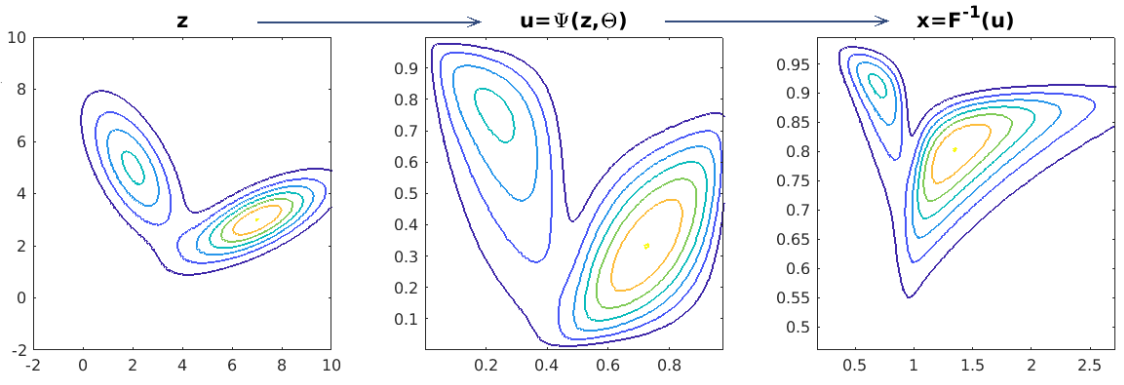
\includegraphics[width=\columnwidth]{figures/figure_gmcm_transformation}}
%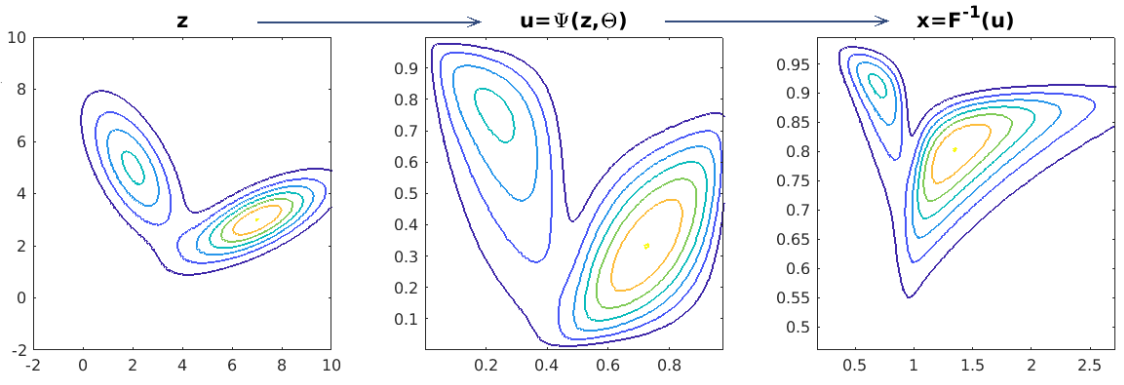
\includegraphics[width= 245pt]{figures/figure_gmcm_transformation}
\caption{Illustration of the transformations induced by a GMCM. The left panel shows the density contours of a 2-component GMM with parameters $\bs{\alpha} = \{0.45, \ 0.55\}$, $\bs{\mu} =\{[2 \ 5], [7 \ 3] \}$ and  $ \Sigma= \{[1.5 \  -1.3 ; -1.3 \quad 3 ],[3 \quad 1.2 ; 1.2 \quad 1] \}$. The middle panel shows the contours under the transformation by the marginal distribution functions [Equation \eqref{eq:invCDF_GMM}]. The right panel shows the transformation  by the quantile functions of $Lognormal(0,0.5)$ and $Beta(10,2)$ distributions along $x$ and $y$ dimensions, respectively. Note that $\bs{x}\in \mathbb{R}_+\times [0,\ 1]$ owing to the Lognormal and Beta marginals.}
\label{fig:gmcm_transformation}
\end{center}
\vskip -0.2in
\end{figure}

\subsection{A numerical scheme to compute $\Psi^{-1}_r(\bs{u}_r;\Theta^r)$} \label{subsec:gmm_quantile}
Section \ref{subsec:MLE_GMCM} emphasized the need for a method to compute $\Psi^{-1}_r(\cdot ;\ \Theta^r)$ that does better than the linear scaling of previous interpolation-based methods. Here, a computationally efficient alternative is proposed where the desired inversion is sought as the root of the expression $\bs{u}_r-\Psi_r(z_r;\Theta^r)$, thus opening door to a rich set of root-finding algorithms. For instance, the well-known \emph{secant-method} enjoys quadratic convergence in most cases \citep{Pedro2003}, thereby needing far less number of function evaluations than the interpolation-based inversion. However, this only partly solves the problem. Since, the partial derivatives of $\Psi^{-1}_r(\cdot;\Theta^r)$ are also needed with respect to $\Theta^r=\{\alpha_l,u_r^l,\sigma_r^l\}_{l=1}^m$. Interestingly, these partial derivatives can be obtained analytically despite the inverse function lacking a closed form. Appendix \ref{apd:gmm_quantile_derivatives} provides the derivation of the aforementioned partial derivatives. PPLs, such as TensorFlow-Probability, allow one to easily embed such custom derivatives so as to allow autodiff to use the same when backpropagating gradients through expression graphs. One may argue the need for analytical derivatives of $\Psi^{-1}_r(\cdot;\Theta^r)$ at all, when PPLs, in principle, can autodiff through iterative, numerical routines such as the secant method. While the argument is correct, autodiff through such routines can easily produce ``...large expression graphs, which can lead to floating point precision errors, excessive memory usage, and slow computation." \citep{Margossian2018}. 

\section{Identifiability of GMCM}\label{sec:identifiability_GMCM}
Another issue that plagues GMCM is that of \emph{unidentifiability}. Identifiability is a key property that determines if a generative model's true parameters can be learned asymptotically with the number of samples. Finite mixture models are known to suffer from the issue of parameter unidentifiability since the likelihood is invariant under a permutation of component labels \citep{Stephens2000}. This is commonly known as \emph{label switching} problem. However, GMCM suffers from another form of parameter unidentifiability as stated in the theorem below.
\begin{theorem}
\label{thm:theorem1}
 Let $U$ be a dataset generated by a $m$-component Gaussian Mixture Copula distribution with true parameters set $\Theta^* = \{\bs{\mu}^{l*}, \Sigma^{l*}, \alpha^{l*}\}_{l=1}^m$. Denote the log-likelihood of the observed data, with respect to the true model, as $\ell_\zeta(\Theta^*|U)$. Define another parameter set $\Theta= \{A\bs{\mu}^{l*}+\bs{b}, \ A^T\Sigma^{l*}A, \ \alpha^{l*}\}_{l=1}^m$, where $A$ is any diagonal positive definite matrix and $\bs{b}$ a real vector. Then, $\ell_\zeta(\Theta|U) = \ell_\zeta(\Theta^*|U)$.
\end{theorem}
Refer to Appendix \ref{apd:Proof_theorem_1} for the proof. A practical repercussion of this result is that the true parameters of a GMC distribution can never be uniquely identified $-$even after addressing the label switching problem$-$ because the likelihood function has infinitely many maximizers. Readers can refer to \citet{White1982} for a detailed exposition on the subject of identifiability in parametric models. \citet{Bilgrau2016} noted this form of non-identifiability in GMCM, although did not prove it. They proposed an ad hoc solution that involved enforcing the first component to have zero mean and unit variance along each dimension. Nevertheless, as noted in their paper, the non-identifiability issue persisted under certain conditions. Here an alternative solution, formalized in Theorem \ref{thm:theorem2}, is proposed that renders GMCM identifiable up to the permutation of component labels.
\begin{theorem}
\label{thm:theorem2} 
Denote $\bs{g}\in \mathbb{R}^d$ and $\bs{h}\in \mathbb{R}_+^d$ as real-valued vectors; the latter being positive. A $m$-component, $d$-dimensional Gaussian Mixture Copula distribution parametrized by $\Theta = \{\bs{\mu}^l, \Sigma^l, \alpha^l\}_{l=1}^m$ is identifiable, up to the permutation of component labels, if and only if the following two conditions are met for any $\bs{g}$ and $\bs{h}$.
\begin{align}
&\sum_{l=1}^m \alpha^l \ \bs{\mu}_r^l=\bs{g}_r \ ,\qquad \forall r \in \{1,2,\cdots,d\} \label{eq:identifiability_constraint_1} \\
&\sum_{l=1}^m \big[ \alpha^l \left(\Sigma_{rr}^l+(\bs{\mu}_r^l)^2\right)\big] -\bs{g}_r^2 =\bs{h}_r ,\qquad \forall r \in \{1,2,\cdots,d\}\label{eq:identifiability_constraint_2}
\end{align}
\end{theorem}
The proof is given in Appendix \ref{apd:Proof_theorem_2}. The choice of $\bs{g}$ and $\bs{h}$ is rather arbitrary. For convenience, the former can be set as $\mathbf{0}^d$ (vector of all zeros) and the latter $\mathbf{1}^d$ (vector of all ones). During the parameter estimation, these constraints can be specified in the form of suitable priors, e.g. Gaussian priors as shown in Equations \eqref{eq:identifiability_prior_1} and \eqref{eq:identifiability_priori_2}, resulting in a well-defined and unique Maximum A Posteriori (MAP) solution. The strength of these priors can be controlled by the parameter $\sigma$ (larger values lead to weaker priors). During experimentation, a value of $\sigma=0.01$ worked well in balancing the trade-off between these priors and the GMCM likelihood.
\begin{align}
& \mathcal{N}\bigl(\sum_{l=1}^m \alpha^l \ \bs{\mu}_r^l \;\ \bs{g}_r,\sigma \bigr),  \label{eq:identifiability_prior_1} \\
&\mathcal{N}\bigl(\sum_{l=1}^m \big[ \alpha^l \left(\Sigma_{rr}^l+(\bs{\mu}_r^l)^2\right)\big] -\bs{g}_r^2 \; \ \bs{h}_r, \sigma \bigr), \label{eq:identifiability_priori_2}\\
&\qquad \qquad \qquad \qquad \qquad \forall r \in \{1,2,\cdots,d\} \nonumber
\end{align}

\section{The EM algorithm for GMCM}\label{sec:EM}
The EM algorithm has garnered popularity for MLE in Gaussian mixture models given that it 1) automatically satisfies the probabilistic constraints and positive definiteness of covariance matrices, 2) doesn't require explicit gradients, and 3) dispenses with the learning rate needed for gradient-based approaches \citep{Xu1996}. The underpinning of EM is a two-step process, the \emph{Expectation} (E)-step that finds a lower bound of the \emph{incomplete data} log-likelihood function (e.g., in Equation \eqref{eq:gmcm_logL}), and the \emph{Maximization} (M)-Step optimizes this lower bound (either partially or fully) to arrive at the next iterate. A repeated application of the E and M steps ensures a monotonic increase of the data log-likelihood until local convergence is achieved. Readers may refer to \citet{Bilmes98agentle} and \citet{Salakhutdinov2002} for detailed treatments on the EM algorithm for GMMs. Although the EM algorithm for GMCMs would follow the same general construct, the E and the M steps are considerably harder than those of GMM. The previous attempts at it \citep{Tewari2011, Bhattacharya2014} do not, systematically, derive and maximize the true lower bound of the incomplete data log-likelihood. Instead, certain assumptions are made that allow tweaking of the GMM's EM algorithm for learning GMCM's parameters. As a result, both of these algorithms need additional checks, at each iteration, to ensure a monotonically increasing likelihood function. They are referred as pseudo-EM (PEM) algorithms for later benchmarking experiments. In summary, a provably correct EM algorithm has remained elusive for GMCM, and this paper closes that gap.
\subsection{E-Step} \label{subsec:EStep}
The ensuing derivation closely follows the exposition in \citet{Bilmes98agentle}, which presents the EM algorithm for GMM in great detail. Assuming access to $\bs{y}$, a $n$-dimensional vector of latent variables that co-occurs with the observed data $U$, the \emph{complete data} log-likelihood function can be written as,
\begin{equation}\label{eq:gmcm_complelte_logL}
\ell_{comp}(\Theta |U,\bs{y})= \sum\limits_{i=1}^{n} \log \left( \frac{\alpha^{\bs{y}_i}\phi \left(\invCDF{:i};\Theta^{\bs{y}_i} \right)}{\llDenom{i}} \right) .
\end{equation}
The latent variable $\bs{y}_i$ denotes the index of the Gaussian component from which the dependence of the $i^{th}$ data sample $U_{:i}$ is derived. The function $\phi(\cdot)$ is the multivariate Gaussian density,  $\Theta^{\bs{y}_i}$ and $\Theta^r$ represent the parameters associated with the component $\bs{y}_i$  and the dimension $r$, respectively. Also, $\invCDF{:i}$ and $Z_{ri}$ are used to denote $\Psi^{-1}\left(U_{:i}\right)$ and $ \Psi_r^{-1}(U_{ri})$, respectively. Note that the denominator does not depend on the latent variable $\bs{y}_i$, since the marginal densities, $\psi_r(\cdot)$ are not component specific. The E-step involves the derivation of the expected value of the complete data log-likelihood (Equation \ref{eq:gmcm_complelte_logL}) with respect to the posterior distribution of the latent variables given the data and the current parameter estimates, say $\hat{\Theta}$. This posterior distribution in this case is $P(\bs{y}|U,\hat{\Theta}) = \prod\limits_{j=1}^{n}P\left(\bs{y}_j|U_{:j},\hat{\Theta} \right)$. Following some tedious but straightforward manipulations (refer to Appendix \ref{apd:EStep_derivation} for details), the expectation of complete data log-likelihood, $Q(\Theta,\hat{\Theta})$, can be written as,
\begin{align}\label{eq:GEM_objective}
Q(\Theta,\hat{\Theta}) =&  \sum\limits_{i=1}^n \sum\limits_{\bs{y}_i=1}^m  \left( \log (\alpha^{\bs{y}_i}) - \frac{\log(|\Sigma^{\bs{y}_i}|)}{2}\right) G_{i\bs{y}^i}  \nonumber \\ 
& -\sum\limits_{i=1}^n \sum\limits_{\bs{y}_i=1}^m  \left( \frac{\zbar{i}^T(\Sigma^{\bs{y}_i})^{-1}\zbar{i}}{2} \right) G_{i\bs{y}^i}  \nonumber \\
& -\sum\limits_{i=1}^n \sum\limits_{r=1}^{d} \log \left(\psi_r(Z_{ri};\Theta^r \right) ,
\end{align}
where $\zbar{i}=Z_{:i}-\mu^{\bs{y}_i}$ is the mean adjusted vector and $G_{i\bs{y}^i}$ is given by Equation\eqref{eq:latent_posterior_matrix}. It should be noted that, unlike the GMM, the E-step in GMCM does not completely remove the logarithm over a sum of exponential terms (see in the third term of Equation \ref{eq:GEM_objective}). Thus, the maximization of \eqref{eq:GEM_objective} does not yield, unlike in the case of GMM, closed-form updates for the model parameters $\Theta$; thereby necessitating a gradient-based M-step. Therefore, it can be argued that the EM algorithm does not enjoy the same benefits for GMCMs \textemdash as it does for GMMs\textemdash over direct likelihood maximization. Nevertheless, the accurately derived E-step can still be maximized (or partially maximized) with a gradient-based M-step while guaranteeing a monotonically increasing incomplete data log-likelihood function (unlike the PEM algorithms proposed in previous works). When the M-step is carried out partially, it would result in a \emph{generalized}-EM (GEM) algorithm, which is compared, in Section \ref{sec:Experimental}, with the aforementioned PEM algorithms.

\section{Experimental Results}\label{sec:Experimental}
This section provides empirical evidence to support the claims made in this paper using synthetic and real-world data sets. The GMCM is coded up in Python using TensorFlow and TensorFlow-Probability primitives.  The experiments aim to convey three key messages, 1) GMCM becomes identifiable in accord with the statement of Theorem \ref{thm:theorem2}, 2) the proposed EM algorithm outperforms the previously published PEM algorithms, and 3) density estimation via GMCM is comparable with the state-of-the-art models on UCI benchmark data sets. For other real-world applications, readers may refer to ~\cite{Bilgrau2012quantification,Wang2014,Yu2013GMCMWindPred,Bayestehtashk2015}, where GMCMs are used for tasks such as prediction, classification, anomaly detection, dependence characterization, etc.

For the first experiment, a 3-dimensional synthetic data set is generated by randomly instantiating an arbitrary 2-component GMC distribution (ground truth). One thousand random samples are generated from this distribution to yield a matrix $U \in [0 \ 1]^{3\times 1000}$, which serves as the training dataset to learn a GMC distribution via direct likelihood maximization. The maximization is carried out using the Adam optimizer \citep{Kingma2014} with the default learning rate of 1E$^{-3}$. The emphasis here is on the ability to recover the parameters of the true data-generating GMC distribution. Figure \ref{fig:identifiability_exp} shows the evolution of the parameters for the two cases; \emph{unregularized} (without the identifiability priors as given by Equations \eqref{eq:identifiability_prior_1} and \eqref{eq:identifiability_priori_2}) and \emph{regularized} (with identifiability priors). Starting from the same initial point, the plots show the evolution of the iterates until numerical convergence (up to 2000 iterations). The green squares show the true GMC parameters. The divergence of iterates from the ground truth is quite apparent for the unregularized case. On the contrary, the iterates converge to the true parameter values for regularized MLE. Although the results are shown only for the mean parameters $\{\bs{\mu}^l \}_{l=1}^3$, the same holds true for other GMC parameters e.g. covariance parameters. Bear in mind that the identifiability priors do not impose any restrictive assumption on the generative process of the data. They are merely making an ill-posed problem (with multiple equivalent solutions), well-posed (with a unique global solution) (see Theorem \eqref{thm:theorem2}).
\begin{figure}[ht]
\vskip 0.2in
\begin{center}
\centerline{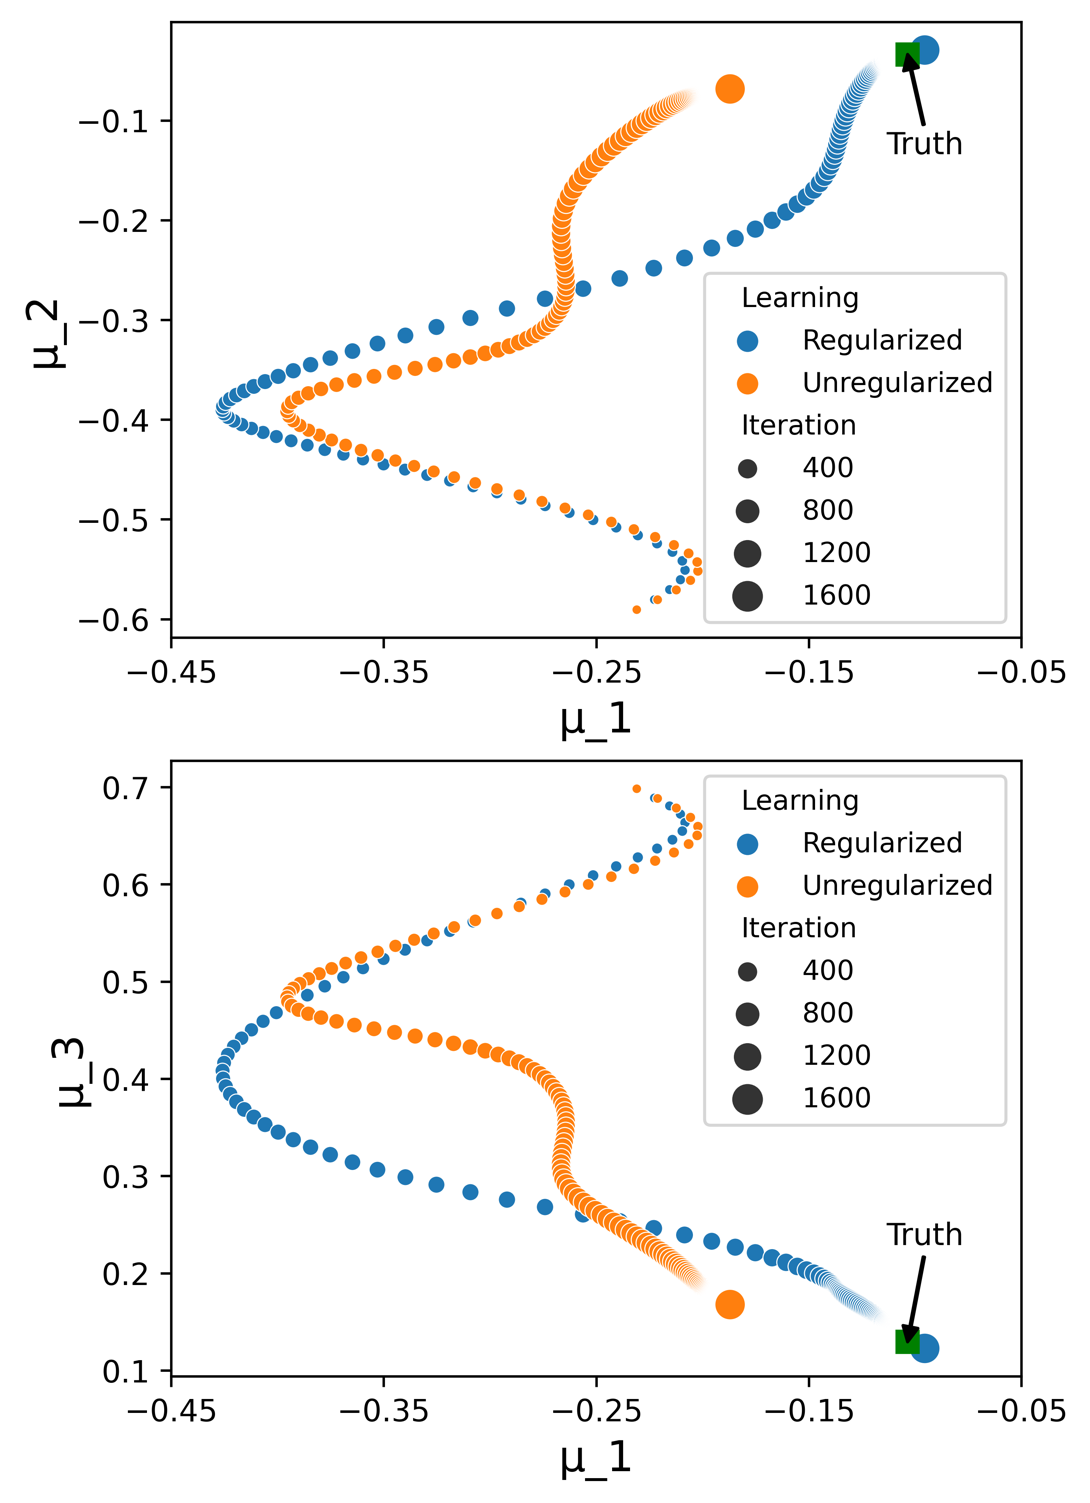
\includegraphics[width= \columnwidth,height=250pt]{figures/Identifiability_Experiment.png}}
\caption{The manifestation of identifiability in GMC distribution is shown empirically. Both plots show the evolution of the mean parameters ($\mu_i$), from the same initial point until numerical convergence (2000 iterations), with and without regularization priors given by Equations \eqref{eq:identifiability_prior_1} and \eqref{eq:identifiability_priori_2}. The true values of the  parameters are shown by green squares.}
\label{fig:identifiability_exp}
\end{center}
\vskip -0.2in
\end{figure} 

The second experiment compares the performance of the proposed generalized EM algorithm with the two pseudo-EM algorithms published in \citet{Bhattacharya2014} and \citet{Tewari2011}, referred to here as PEM$_1$ and PEM$_2$, respectively. The key performance indicator here is the log-likelihood value attained at the convergence of these algorithms. To ensure an exhaustive comparison, 100 datasets are generated by following the same procedure as in experiment 1. For each dataset, the GMC parameters are learned by the three algorithms with identical initialization. Figure \ref{fig:EM_algo_comp}(a) plots the log-likelihood vs. iteration, from the three algorithms, for one such dataset. GEM can be seen to converge to a higher log-likelihood value compared to PEM$_1$ and PEM$_2$. This observation is quite consistent over other datasets. Figure \ref{fig:EM_algo_comp}(b) summaries the results over all the datasets by showing the box-plots of the log-likelihood ratios, $\log\left( \frac{\mathcal{L}\left(\Theta^{GEM}|U\right)}{\mathcal{L}\left(\Theta^{PEM_1}|U\right)}\right)$ and $\log\left( \frac{\mathcal{L}\left(\Theta^{GEM}|U\right)}{\mathcal{L}\left(\Theta^{PEM_2}|U\right)}\right)$, of the converged models. A significantly positive median and the quantile values confirm the superior performance of GEM over PEM$_1$ and PEM$_2$.
\begin{figure}[ht]
\vskip 0.2in
\begin{center}
\centerline{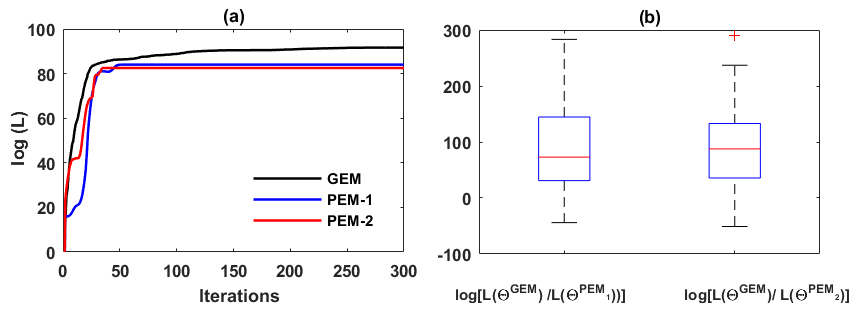
\includegraphics[width=\columnwidth,keepaspectratio=true]{figures/EM_algo_comparisons}}
\caption{(a) log-likelihood vs. iteration for the three EM algorithms on a simulated dataset (b) Box-plots of converged log-likelihood ratios,  $\log\left( \frac{\mathcal{L}\left(\Theta^{GEM}|U\right)}{\mathcal{L}\left(\Theta^{PEM_1}|U\right)}\right)$ and $\log\left( \frac{\mathcal{L}\left(\Theta^{GEM}|U\right)}{\mathcal{L}\left(\Theta^{PEM_2}|U\right)}\right)$, by repeating this experiment on 100 such simulated datasets. The sub-optimal performance of PEM algorithms is clearly evident.}
\label{fig:EM_algo_comp}
\end{center}
\vskip -0.2in
\end{figure}  

Finally, GMCM is learned on several density estimation benchmarks from the UCI repository, after following the pre-processing step described in \citep{Papamakarios2017}. The test log-likelihoods of GMCM with several other marginalizable and non-marginalizable density models are presented in Table \ref{tab:DE_results_UCI}. In order to have the same complexity, the mixture models (GMCM and GMM) were instantiated with the 40 mixing components. This number was ascertained by a grid search over {10,20,30,40,50} and tracking the likelihood of validation data sets. The test log-likelihood numbers for the other models are lifted from other benchmark studies \citep{Papamakarios2017, Gilboa2021}. The performance of GMCM is found to be comparable and better (on higher dimensional data sets) than its marginalizable counterparts. However, the non-marginalizable variants clearly have superior performance, but at the cost of losing the ability to marginalize. Nevertheless, the goal here is not to prescribe one modeling framework over the other (that choice is largely application dependent), but rather to establish GMCM as a useful addition to data modelers' repertoire of tools. Moreover, average log-likelihood is only one of the metrics for model evaluation and need not imply good performance on the task at hand \citep{Theis2015}.
\begin{table}[t] \label{tab:DE_results_UCI}
\caption{Average test log-likelihood achieved by different density estimation models on UCI benchmark data sets. The models are grouped as \emph{non-marginalizable} (top panel) and \emph{marginalizable} (bottom panel). The best-performing model for each group and data set is shown in bold. Error bars correspond to two standard deviations.}
\label{yyyy}
\vskip 0.15in
\begin{center}
\begin{small}
\begin{sc}
\resizebox{\columnwidth+0.1in}{!}{%
\begin{tabular}{lcccr}
\toprule
\textbf{non-Marg.} & \textbf{Power}  & \textbf{Gas} & \textbf{Hepmass} & \textbf{Miniboone} \\
\midrule
Kingma 2018         & 0.17 ± .01               & 8.15 ± .40               & -18.92 ± .08                & -11.35 ± .07                  \\
Grathwohl 2019      & 0.46 ± .01               & 8.59 ± .12              & -14.92 ± .08                & -10.43 ± .04                  \\
Huang 2018          & 0.62 ± .01               & 11.96 ± .33             & -15.08 ± .40                 & -8.86 ± .15                   \\
Oliva 2018          & 0.60 ± .01               & \textbf{12.06 ± .02}    & -13.78 ± .02                & -11.01 ± .48                  \\
De Cao 2019         & 0.61 ± .01               & 12.06 ± .09             & -14.71 ± .38                & -8.95 ± .07                   \\
Bigdeli 2020        & 0.97 ± .01               & 9.73 ± 1.14             & \textbf{-11.3 ± .16}        & \textbf{-6.94 ± 1.81}                 \\
Gilboa 2021         & \textbf{1.78 ± .12}      & 8.43 ± .04              & -18.0 ± 0.91                & -18.6 ± .47          \\        
\bottomrule
\textbf{Marg.} & \textbf{Power}  & \textbf{Gas} & \textbf{Hepmass} & \textbf{Miniboone} \\
\midrule
Gaussian          & -7.74 ± .02         & -3.58 ± .75            & -27.93 ± .02          & -37.24 ± 1.07                  \\
GMM               & -0.26 ± .03         & 5.85 ± .11             & -20.65 ± .88          & -23.83 ± 1.09                  \\
GMCM              & 0.13 ± .02          & 6.10 ± .04             & \textbf{-16.39 ± .52} & \textbf{-22.65 ± .12}                   \\
Gilboa 2021       & \textbf{0.57 ± .01} & \textbf{8.92 ± .11}    & -20.08 ± .06          & -29.01 ± .06                  \\
\bottomrule
\end{tabular}}
\end{sc}
\end{small}
\end{center}
\vskip -0.1 in
\end{table}
\section{Discussion}\label{sec:Discussion}
This paper addresses a few outstanding issues with the estimation of GMCM parameters that have been impeding its use as a mainstream data modeling tool, despite its superior expressivity yet similar intuitivity to the widely used GMM. The first one is that of parameter unidentifiabilty which has been well-acknowledged but loosely addressed in previous works. The proposed identifiability priors mitigate this issue in a principled manner. The second issue pertains to the intractability of GMCM's likelihood (due to the lack of closed-form quantile function of a univariate mixture of Gaussians). While this inherent issue persists, a superior numerical scheme and the associated analytical partial derivatives, presented in this paper, go a long way to make the MLE of GMCM computationally efficient. Lastly, the paper also presents a provable correct \emph{generalized}-EM algorithm for GMCM. Previous attempts at it, proposed parameter update rules that do not maximize the true lower bound of the GMCM log-likelihood. As a result, additional checks and corrections were needed to ensure a monotonically increasing log-likelihood during EM updates. The paper also argues that the GMCM does not enjoy the same benefits, as the GMM, from the EM algorithm, thereby prescribing direct likelihood maximization with suitable parameterization.   

An interesting unexplored aspect pertains to the Bayesian parameter estimation of GMCM. Previously unidentifiability of GMCM would have caused performance issues in posterior approximations via both sampling or variational inference methods. How well the proposed identifiability priors (Equations \eqref{eq:identifiability_prior_1} and \eqref{eq:identifiability_priori_2}) improve the performance of posterior approximation methods remains to be seen. Another research direction would be to investigate the GMCM behavior under conditioning operation. Although GMCM is closed under marginalization, it need not be closed under conditioning. The latter would be a useful property for regression applications of GMCM.  A remaining direction would be to induce sparsity in the precision matrices of the Gaussian components. This would bring significant benefits in high-dimensional settings where the data for training is scarce, and there's a significant risk of over-training. 

%\section*{\refname}

% In the unusual situation where you want a paper to appear in the

% references without citing it in the main text, use \nocite

%\nocite{langley00}

\bibliography{citations}
\bibliographystyle{icml2023}

 

%%%%%%%%%%%%%%%%%%%%%%%%%%%%%%%%%%%%%%%%%%%%%%%%%%%%%%%%%%%%%%%%%%%%%%%%%%%%%%%
%%%%%%%%%%%%%%%%%%%%%%%%%%%%%%%%%%%%%%%%%%%%%%%%%%%%%%%%%%%%%%%%%%%%%%%%%%%%%%%
% APPENDIX
%%%%%%%%%%%%%%%%%%%%%%%%%%%%%%%%%%%%%%%%%%%%%%%%%%%%%%%%%%%%%%%%%%%%%%%%%%%%%%%
%%%%%%%%%%%%%%%%%%%%%%%%%%%%%%%%%%%%%%%%%%%%%%%%%%%%%%%%%%%%%%%%%%%%%%%%%%%%%%%

\newpage
\appendix
\onecolumn
\section{Glossary of frequently used symbols} \label{apd:symbol_glossary}
\begin{table}[h]
\caption{Symbols and descriptions}
\label{tab:symbol_glossary}
\begin{tabular}{ll}
\hline
\textbf{Symbol} & \textbf{Description} \\
\hline
$d$ & data dimensions \\
$m$ & number of components in the mixture model \\
$n$ & number of data samples \\
$\Theta = \{\bs{\mu}^l, \Sigma^l, \alpha^l\}_{l=1}^m$ & parameter of $m$-component, $d$-dimensional GMM \\
$\Theta^r= \{\bs{\mu}_r^l, \Sigma_{rr}^l, \alpha^l\}_{l=1}^m$ & parameters of marginal GMM along the $r^{th}$ dimension $(\Theta^r \subset \Theta)$ \\
$f_r $ & arbitrary univariate density function \\
$F_r, F_r^{-1}$ & the distribution and the quantile function corresponding to $f_r$ \\
$F$ & vector function defined as $F = [F_1, F_2,\cdots,F_d]$ \\
$\psi, \Psi$ & joint density and distribution function of GMM in $\mathbb{R}^d$ \\
$\psi_r , \Psi_r$ & density and distribution function of the of the GMM along the $r^{th}$ dimension \\
$\Psi_r^{-1}$ & quantile function corresponding to $\Psi_r$ \\
$\Psi^{-1}$ & vector function defined as $\Psi^{-1} = [\Psi_1^{-1}, \Psi_2^{-1},\cdots,\Psi_d^{-1}]$ \\
$\bs{x} \in \mathbb{V}^d$ & real valued vector whose distribution is sought \\
$\bs{u} \in [0,1]^d=F(\bs{x})$ &  vector of uniformly distributed random variables \\
$\bs{z} \in \mathbb{R}^d =\Psi^{-1}(\bs{u}) $ &  vector with quantile values of GMM marginals \\
$X \in \mathbb{V}^{d \times n}$ & matrix of $n$, $\bs{x}$ vectors arranged columnwise \\
$U \in [0,1]^{d \times n}$ & matrix of $n$, $\bs{u}$ vectors arranged columnwise \\
$Z \in \mathbb{R}^{d \times n}$ & matrix of $n$, $\bs{z}$ vectors arranged columnwise \\
$\bs{y}$ & $n$-dimensional vector such that $\bs{y}_i \in \{1,2,\cdots,m\}$ \\
\hline
\end{tabular}
\end{table}

\section{Proofs}\label{apd:Proofs}
\subsection{Theorem 1}\label{apd:Proof_theorem_1}
\textbf{Proof}:  Let $\bs{z}\in \mathbb{R}^d$ is drawn from a $m$-component Gaussian mixture distribution with parameters $\Theta^* = \{\bs{\mu}^{l*}, \Sigma^{l*}, \alpha^{l*}\}_{l=1}^m$. Define strictly increasing transformations i.e. $\bs{w}_r = a_r \bs{z}_r+b_r$, with $a_r \in \mathbb{R}^+$ and $b_r \in \mathbb{R}$. Then $\bs{w}= [\bs{w}_1, \bs{w}_2,\ldots \bs{w}_d]$  has a Gaussian mixture distribution with parameters  $\Theta= \{A\bs{\mu}^{l*}+\bs{b}, \ A^T\Sigma^{l*}A, \ \alpha^{l*}\}_{l=1}^m$, where $A = \text{diag}([a_1, a_2, \cdots a_d])$ and $\textbf{b}=[b_1, b_2, \cdots b_d]$.

The vector $\bs{u}\in [0,1]^d$, such that $\bs{u}_r = \Psi_r(\bs{z}_r;\Theta^{*r}); r=1,2,\cdots, d $, has the joint density function (see definition 2 of GMC distribution) given by equation \eqref{eq:true_GMC_density}.
\begin{align}\label{eq:true_GMC_density}
\zeta(\bs{u};\Theta^*) & = \left( \frac{\psi\left(\bs{z};\Theta^*\right)}{\prod\limits_{r=1}^{d}\psi_r\left(z_r;\Theta^{r*} \right)} \right)
\end{align}
Likewise, the density function of $\bs{v}\in [0,1]^d$ such that $\bs{v}_r = \Psi_r(\bs{w}_r;\Theta^r); r=1,2,\cdots, d $ has the density function given by equation \eqref{eq:transformed_GMC_density}.
\begin{align}\label{eq:transformed_GMC_density}
\zeta(\bs{v};\Theta) & = \left( \frac{\psi\left(\bs{w};\Theta\right)}{\prod\limits_{r=1}^{d}\psi_r\left(\bs{w}_r;\Theta^r \right)} \right)
\end{align}
However, since cumulative distribution function values remain invariant under strictly increasing transformations, we have $\bs{u} \equiv \bs{v}$. This means $\bs{u}$ and $\bs{v}$ have the same generative distribution, or equivalently $\zeta(\textbf{u};\Theta^*) = \zeta(\textbf{u};\Theta)$. Therefore, the corresponding likelihood functions, defined on a dataset with $n$ samples $(U \in [0 , 1]^{d\times n})$, are equal for the two parameter configurations $\Theta^*$ and $\Theta$ i.e. $\ell_\zeta(\Theta|U) = \ell_\zeta(\Theta^*|U)$. This completes the proof.

\subsection{Theorem 2} \label{apd:Proof_theorem_2}
\textbf{Proof}: The proof is straightforward in the light that the LHS expression in Equations \eqref{eq:identifiability_constraint_1} and \eqref{eq:identifiability_constraint_2} correspond to the mean and the variance of the marginals of a GMM, respectively. Affixing the vectors $\bs{g}$ and $\bs{h}$ to pre-specified values, therefore, prohibits the transformations that cause non-identifiability  (refer to Theorem \ref{thm:theorem1}). Intuitively, by fixing the margins of the GMM (as we only seek the dependence structure it encodes), we eliminate different parameter configurations that encode the same dependence structure. Conversely, any parameter update that abides by the constraints specified in Theorem 2, would result in non-increasing transformations, thus mitigating the non-identifiability noted in Theorem \ref{thm:theorem1}.

%\section{Derivation of E-Step}\label{apd:EStep_derivation}
%Let's denote the posterior distribution on the latent variables, given the current iteration $\hat{\Theta}$, as $P(\bs{y}|U,\hat{\Theta}) = \prod\limits_{j=1}^{n}P\left(\bs{y}_j|U_{:j},\hat{\Theta} \right)$.  The expectation of the complete data log-likelihood in Equation \eqref{eq:gmcm_complelte_logL}, with respect to $P(\bs{y}|U,\hat{\Theta})$,  can be written as
%\begin{align} \label{eq:ll_comp_expectation}
%Q(\Theta,\hat{\Theta})&=\sum\limits_{\bs{y}^1=1}^m \ldots \sum\limits_{\bs{y}^n=1}^m \left[ \left( \sum\limits_{i=1}^{n}H_{i\bs{y}_i}  \right) \prod\limits_{j=1}^{n}G_{j\bs{y}_j} \right] \text{  where,}
%\end{align}
%\begin{align}
%H_{i\bs{y}_i} &= \log \left(\frac{\alpha^{\bs{y}_i}\phi(\invCDF{:i}; \Theta^{\bs{y}_i})}{\llDenom{i}} \right),\quad\text{and}\quad
%G_{j\bs{y}_j} = P\left(\bs{y}_j|U_{:j},\hat{\Theta}\right) \nonumber
%\end{align}
%with $H$ and $G$ being matrices of dimensions $n\times m$. The $(j,l)^{th}$ element of the matrix $G$ denotes the posterior probability of the $l^{th}$ component given the $j^{th}$ sample and the current parameter estimate $\hat{\Theta}$, and is computed as
%\begin{align}
%G_{jl}=P\left(\bs{y}^j=l|U_{:j},\hat{\Theta}\right)=\frac{\alpha^l\phi\left(\Psi^{-1}(U_{:j}); \hat{\Theta}^l\right)}{\sum_{i=1}^m\alpha^i\phi\left(\Psi^{-1}(U_{:j}); \hat{\Theta}^i\right)}.
%\end{align}

\section{Derivation of E-step}\label{apd:EStep_derivation}
Let's denote the posterior distribution on the latent variables, given the current iteration $\hat{\Theta}$, as $P(\bs{y}|U,\hat{\Theta}) = \prod\limits_{j=1}^{n}P\left(\bs{y}_j|U_{:j},\hat{\Theta} \right)$.  The expectation of the complete data log-likelihood in Equation \eqref{eq:gmcm_complelte_logL}, with respect to $P(\bs{y}|U,\hat{\Theta})$,  can be written as
\begin{align} \label{eq:ll_comp_expectation}
Q(\Theta,\hat{\Theta})=\sum\limits_{\bs{y}^1=1}^m \sum\limits_{\bs{y}^2=1}^m \ldots \sum\limits_{\bs{y}^n=1}^m \left[ \left( \sum\limits_{i=1}^{n}H_{i\bs{y}^i}  \right) \prod\limits_{j=1}^{n}G_{j\bs{y}^j} \right] \text{  where,}
\end{align}
\begin{align*}
H_{i\bs{y}^i} &= \log \left(\frac{\alpha^{\bs{y}^i}\phi(\invCDF{:i}; \Theta^{\bs{y}_i})}{\llDenom{i}} \right),\quad\text{and}\quad
G_{j\bs{y}^j} = P\left(\bs{y}^j|U_{:j},\hat{\Theta}\right) \nonumber
\end{align*} 
The $(j,l)^{th}$ element of the matrix $G$ denotes the posterior probability of the $l^{th}$ component given the $j^{th}$ sample and the current parameter estimate $\hat{\Theta}$, and is computed as
\begin{align} \label{eq:latent_posterior_matrix}
G_{jl}=P\left(\bs{y}^j=l|U_{:j},\hat{\Theta}\right)=\frac{\alpha^l\phi\left(\Psi^{-1}(U_{:j}); \hat{\Theta}^l\right)}{\sum_{i=1}^m\alpha^i\phi\left(\Psi^{-1}(U_{:j}); \hat{\Theta}^i\right)}.
\end{align}
The expression in \ref{eq:ll_comp_expectation} can be expanded to obtain,
\begin{align}
Q(\Theta,\hat{\Theta}) &= \sum\limits_{\bs{y}^1=1}^m H_{1\bs{y}^1}G_{1\bs{y}^1} \prod\limits_{j=1,j\neq 1}^n \sum\limits_{\bs{y}^j=1}^m G_{j\bs{y}^j} \nonumber \\
& + \sum\limits_{\bs{}^2=1}^m H_{2\bs{y}^2}G_{2\bs{y}^2)}\prod\limits_{j=1,j\neq 2}^n \sum\limits_{\bs{y}^j=1}^m G_{j\bs{y}^j} + \ldots  \nonumber \\ 
& \ldots + \sum\limits_{\bs{y}^n=1}^m H_{n\bs{y}^n}G_{n\bs{y}^n}\prod\limits_{j=1,j\neq n}^n \sum\limits_{\bs{y}^j=1}^n G_{j\bs{y}^j}
\end{align}
Given that $\sum\limits_{\bs{y}^j=1}^m G_{j\bs{y}^j} = 1, \text{ for all }  j \in \{1,\ldots, n\} $, the above equation simplifies as.
\begin{equation} \label{eq:simplflied_expectation}
Q(\Theta,\hat{\Theta}) = \sum\limits_{i=1}^{n}\sum\limits_{\bs{y}^i=1}^m H_{i\bs{y}^i}G_{i\bs{y}^i}.
\end{equation}
Thereafter, it is easy to establish 1-to-1 correspondence between Equations \eqref{eq:simplflied_expectation} and \eqref{eq:GEM_objective} by expanding the term $H_{i\bs{y}^i}$.

\section{Partial derivatives of $\Psi^{-1}_r(\cdot)$}\label{apd:gmm_quantile_derivatives}
Let's say that $z_r=\Psi_r^{-1}(u)$. Even though $\Psi^{-1}_r(\cdot)$ does not have a closed-form, its partial derivatives can be obtained analytically via its forward function $\Psi_r(\cdot)$, and by invoking Euler's chain rule, as shown in Equation \eqref{eq:TripleProduct}.
\begin{equation}\label{eq:TripleProduct}
\frac{dz_r}{d\theta}=- \frac{\left(\frac{d\Psi_r(z_r)}{d\theta}\right)_z}{\left(\frac{d\Psi_r(z_r)}{dz_r}\right)_\theta}
\end{equation}
The expression in the denominator is identical for all the partial derivatives and is simply the density functionof the univariate GMM, i.e 
\begin{equation}\label{eq:Gamma_dz}
\der{z_r}{\Psi_r(z_r)}=\psi_r(z_r).
\end{equation}
The partial derivatives of the numerator can be derived, as follows, by applying of matrix calculus identities.
\\
\text{Derivative of $z_r$ w.r.t to $\alpha_k$}
\begin{equation}
\der{\alpha_k}{\Psi_r(z_r)}=\frac{1}{2}\left[1+ \erf \left( \frac{z_r-\mu_{k,r}}{\sqrt{2\Sigma_{r,k}}}\right) \right]
\end{equation}
\\
\text{Derivative of $z_r$ w.r.t to $\mu_k$}
\begin{equation}
\der{\mu_k}{\Psi_r(z_r)}= -\frac{\alpha_k}{\sqrt{2\pi\Sigma_{r,k}}}\exp\left( - \frac{(z_r-\mu_{k,r})^2}{2\Sigma_{r,k}}	 \right)
\end{equation}
\\
\text{Derivative of $z_r$ w.r.t to $\Sigma_k$}
\begin{equation}
\der{\Sigma_k}{\Psi_r(z_r)}= -\sum\limits_{l=1}^{m}\frac{\alpha_l}{\sqrt{2\pi\Sigma_{r,l}}}\exp\left( - \frac{(z_r-\mu_{r,l})^2}{2\Sigma_{r,l}} \right) \times \frac{(z_r-\mu_{r,l})}{2\Sigma_{r,l}} \times \der{\Sigma_k}{\Sigma_{r,l}}
\end{equation}
\end{document}